\chapter{Analýza a návrh řešení}
% Analýza a návrh implementace (včetně diskuse různých alternativ a volby implementačního prostředí).
% Detailní popis uživatele a jeho potřeb.
% Analýzu odkázat na komparativní test.
% Návrh odkázat na low fidelity test.
% V analýze neprezentovat finální řešení ale dopodrobna celý proces.

% Vytvořte mobilní navigační systém po elektrotechnické fakultě ČVUT.
% Systém musí co nejlépe sloužit svému účelu a vyhovovat potřebám typického uživatele -- studenta. Je nutné, aby vhodným způsobem naváděl uživatele k cílovému bodu a byl spustitelný na co největším počtu současných mobilních zařízení. Systém umožní lokalizaci zadaného cílového místa (konkrétní učebnu, nejbližší toalety...) a dokáže do něj najít optimální cestu ze zadaného výchozího bodu. Vytvořenou aplikaci testujte s uživateli a zohledněte zjištěné problémy.


Analýze problematiky byla věnována přibližně polovina času vyměřeného na tuto práci. Do tohoto času je započítáno všechno, co se zkoumání dané problematiky týká, tedy zjišťování potřeb uživatelů, tvorba a evaluace prototypů, sestavení případů užití a komplementace požadavků. Do této kapitoly byl zařazen i návrh.

Vývoj probíhal částečně vodopádovým (z organizačních důvodů bylo potřeba dopředu stanovit některé termíny) a spirálovým modelem (tím se řídil zbytek) a v postupných iteracích se měnily a přidávaly nové požadavky -- to je hlavním důvodem umožnění tak podrobné analýzy.

Následující sekce chronologicky odpovídají postupu vývoje, nikdy ale nedošlo přestupem do další fáze k úplnému ukončení té předchozí, vždy se k ní vývoj při další iteraci zase stočil.

\section{Potřeby uživatelů}
Tato sekce slouží jako seznam potřeb uživatelů, se kterými jsem se v průběhu práce setkal. Ne všechny potřeby byly později zapracovány do výsledné aplikace, některé totiž nebyly natolik důležité, aby se je vyplatilo v aplikaci mít a zastiňovat jimi potřeby důležitější. Další potřeby bývaly protichůdné a také je nešlo implementovat zároveň. Popisu uživatele se věnuje už sekce \ref{sec:popisUzivatele}.

\subsection{Potřeba se někam dostat}
Touto potřebou se zabývá celá práce. Student zná označení místnosti (nebo i méně exaktní identifikátor), ale neví, kde se daná místnost nachází, ani kudy se k ní dostat. 

Hledaná místa mohou být různá, může to být třeba:
\begin{itemize}
\item učebna (ve které má student výuku nebo zkoušku),
\item kancelář vyučujícího (ke kterému si jde pro známku z předmětu nebo na konzultaci),
\item toalety (nejbližší nebo třeba nejméně frekventované),
\item občerstvení (nejbližší automat nebo bufet s velkým sortimentem),
\item hasící přístroj (jeho potřeba není častá, takže se jím dále nebudeme zabývat),
\item únikový východ (také se jím, ze stejných důvodů, nebudeme zabývat),
\item vrátnice (ta se ale hledá svou výlučnou přítomností u vchodu do budovy snadno),
\item další takzvané body zájmu.
\end{itemize}

Lokalizace hledaného místa může být provedena při znalosti:
\begin{itemize}
\item označení místnosti (KN:E-107), pokud hledáme učebnu a známe ho třeba z rozvrhu,
\item starého označení (K1), pokud nám někdo řekne označení z doby před přečíslováním,
\item oficiálního názvu místnosti (Zengerova posluchárna),
\item neoficiálního názvu místnosti (Solárium, Bouračka, Bufet\dots),
\item jména vyučujícího, pokud hledáme jeho kancelář,
\item umístění vchodu do budovy, pokud třeba hledáme vrátnici,
\item polohy všech míst, které přicházejí v úvahu (třeba bufetů), nebo to a navíc ještě
\item přibližné aktuální polohy, pokud hledáme něco nejbližšího.
\end{itemize}

\subsection{Potřeba určit polohu místa}
Nejprve je nutné zjistit polohu místa, kam se potřebujeme dostat\footnote{Teoreticky je možné polohu neznat a tupě se řídit shora podávanými instrukcemi, toto řešení ale není lidské mentalitě příjemné a proto se jím práce nezabývá.} a až poté má smysl se zamýšlet nad samotnou cestou. Poloha se dá s předchozími zkušenostmi odhadnout,\footnote{Například poloha místnosti se dá odhadnout z jejího názvu, který sám o sobě identifikuje budovu a~podlaží.} předchozí zkušenosti ale nejsou zaručeny a správný odhad teprve ne.

K přesnému určení místa se dá dospět několika způsoby:
\begin{itemize}
\item náhodným zkoušením, to ale nebývá optimální,
\item přeptáním se, to ale dělá, často introvertním, studentům problémy,
\item vyhledáním v mapě, pokud je k dispozici.
\end{itemize}

\subsection{Potřeba určit cestu k místu}
Teprve tehdy, až známe polohu hledané místnosti, k ní můžeme začít určovat cestu. Způsoby jsou stejné jako u hledání místa samotného -- zkoušení, přeptávání a vyhledání na~mapě. 

\subsection{Potřeba navigační aplikace}
Všechny předchozí potřeby by se daly uspokojit vhodnou aplikací -- ta dokáže určit polohu místa a nalézt k němu cestu pro uživatele velmi komfortně. Aplikaci je nicméně potřeba vytvořit a je potřeba to udělat pořádně -- tím se zabývají následující potřeby, jinak bude pro~uživatele lepší se i nadále spoléhat na svou intuici.

\subsection{Potřeba mobilní aplikace}
Místnost je dost často potřeba najít okamžitě, několik minut předtím, než v ní máme být. V této době není čas shánět se po počítači, navíc už můžeme být v pohybu předpokládaným směrem. Z toho plyne potřeba aplikace mobilní.

Studenti Fakulty elektrotechnické, kterými se práce zabývá, zpravidla tíhnou k technickým hračkám, například k mobilním telefonům a tím pádem i jejich aplikacím, více, než většina populace. Dá se tedy předpokládat, že mobilní telefony mají, a dá se předpokládat i~to, že budou tyto telefony schopny provozovat jednoduchou navigační aplikaci.

\subsection{Potřeba použitelné aplikace}
Aby aplikaci vůbec někdo používal, je nutné, aby byla použitelná, aby se s ní dalo pracovat i bez návodu a vše bylo přehledné. Je dobré, když aplikace umožňuje vyhledávat i~bez diakritiky, nerozlišuje při vyhledávání velikost písmen, umožní zadat regulární výraz pro~nalezení místa s ne úplně přesně známým názvem a podobně.

\subsection{Potřeba korespondující navigace aplikace se skutečností}
Je nutné, aby se dokázal uživatel podle aplikace někam dostat. Musí se nejprve zorientovat, zjistit kam se chce dostat a kudy se tam dostat. V těchto krocích mu musí aplikace pomáhat.

\subsection{Potřeba multiplatformní aplikace}
Mobilní zařízení jsou specifická svými implementacemi standardů, dost často jsou tyto implementace, pokud jsou vůbec přítomny, pro nedostatek prostředků poskytovaných zařízením osekané a někdy i od standardů odlišné. Není to ideální, ale je to pochopitelné. Bohužel je ale nepřeberné množství zařízení a téměř u každého modelu je něco jinak, než jinde. Je pak v některých případech velmi těžké nalézt multiplatformní řešení.

\subsection{Potřeba aktuálního obsahu aplikace}
Obsah aplikace by měl být aktuální a reflektovat stávající situaci: uzavírky, přestavby a~jiné mimořádné události. Aplikace může čerpat některá aktuální data z \url{http://udb.feld.cvut.cz}, například označení místnosti, ve které má student podle rozvrhu následující hodinu, nebo kanceláře vyučujícího. Navede-li aplikace někoho špatně, aktuálně opravovanou, slepou cestou, riskuje se ztráta uživatele.

\subsection{Potřeba offline provozu aplikace}
Částečně v rozporu s předchozím bodem je potřeba offline provozu aplikace. Mnoho studentů ještě nemá ve svých mobilních zařízeních možnost připojení k Internetu a o ty by aplikace online provozem přišla. Aplikace by tedy měla zvládat práci offline, ale také by mohla umožňovat online provoz a aktualizace pro offline provoz.

\subsection{Potřeba navedení optimální cestou aplikací}
\label{subs:UNcestaAplikaci}
Hledání optimální cesty je poměrně složitá záležitost, ačkoliv se to na první pohled nezdá. Optimální cesta není ta nejkratší nebo nejrychlejší, je to mnohem složitější. Do hry vstupuje mnoho kritérií, například:
\begin{itemize}
\item délka cesty -- má být většinou nejkratší,
\item doba cesty -- má být většinou nejkratší,
\item terén -- tady už začínají komplikace, někdo se rád projde po schodech, jiný může mít zlámanou nohu, tak chce jet páternosterem a další je na vozíčku, předchozí způsoby nemůže využít a musí jet obyčejným výtahem,
\item zapamatovatelnost cesty -- má být většinou nejsnazší,
\item frekventovanost -- někteří se rušným cestám vyhýbají, jiní je vyhledávají,
\item místa kolem cesty -- někteří raději nevolí cestu kolem kanceláří neoblíbených vyučujících...
\end{itemize}
Na první pohled je jasné, že téměř nikdy nemůže existovat cesta, která by byla ve všech zmiňovaných kritériích nejlepší. Je nevděčné vytvářet univerzálně nejlepší cestu a nad lidské síly sestavovat optimální algoritmus pro zjištění individuálně nejlepší cesty; vytvořit použitelnou implementaci v omezeném mobilním prostředí tedy bohužel asi nepůjde.

\subsection{Potřeby návštěvníků na aplikaci}
Návštěvníci mají specifické potřeby na aplikaci. Zajímavé by mohlo třeba být prozkoumat potřeby potencionálních studentů, kteří se jdou podívat na den otevřených dveří, a~poskytnout jim aplikaci jako průvodce mezi jednotlivými stanovišti dne otevřených dveří. Zadání práce ale vymezuje cílovou skupinu jako studenty FELu, takže se těmito potřebami nebudeme dále zabývat.



\section{Prototypy}
Po ujasnění několika základních potřeb a požadavků jsem začal vytvářet prototypy. Nejprve pouze jednoduché low fidelity prototypy pro vyjasnění základních požadavků, později sofistikovanější high fidelity prototypy reprezentující chování i vzhled výsledné aplikace.

\subsection{Low fidelity prototypy}
Low fidelity prototypy jsou, většinou papírové, snadno vytvořitelné prototypy, na kterých se navrhují a testují některé základní aspekty aplikace -- rozvržení komponent, jednoduchá interakce, návaznost akcí a podobně. Mají tu výhodu, že zadavateli přiblíží finální aplikaci, udělá si konkrétnější představu a lépe se mu pak formulují požadavky.

Za pomoci low fidelity prototypů se vymezily jednotlivé obrazovky aplikace. Výchozí obrazovka je v podstatě jedinou nutnou obrazovkou aplikace, obsahuje menu pro přechod do dalších obrazovek, vyhledávací formulář a krátkou nápovědu. Dalšími obrazovkami jsou nápověda, nápověda regulárních výrazů a obrazovka se základními informacemi o programu.

Nejvýznamnějším ovládacím prvkem bude velké vyhledávací pole uprostřed úvodní obrazovky -- uživatel zde bude moci zadat všechno, co potřebuje nalézt, a aplikace by mu to měla vyhledat. V případě, že bude nalezeno více výsledků, zobrazí se jejich seznam (viz obrázek~\ref{fig:LFviceVysledku}\footnote{Low fidelity prototypy byly vytvořeny v nástroji Balsamiq Mockups \cite{BalsamiqMockups}.}), ze kterého si bude moci uživatel vybrat nebo upřesnit hledaný výraz, jinak se navede rovnou k cíli (viz obrázek~\ref{fig:LFjedinyVysledek}).

\begin{figure}[ht]
\begin{center}
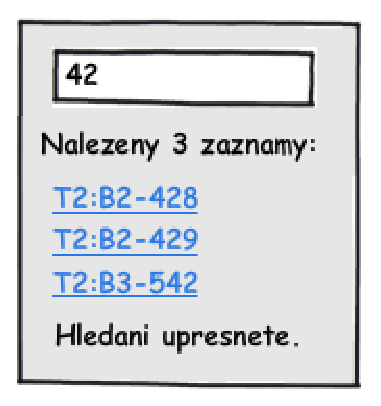
\includegraphics[width=30mm]{figures/LFviceVysledku}
\caption{Nalezení několika výsledků}
\label{fig:LFviceVysledku}
\end{center}
\end{figure}

\begin{figure}[ht]
\begin{center}
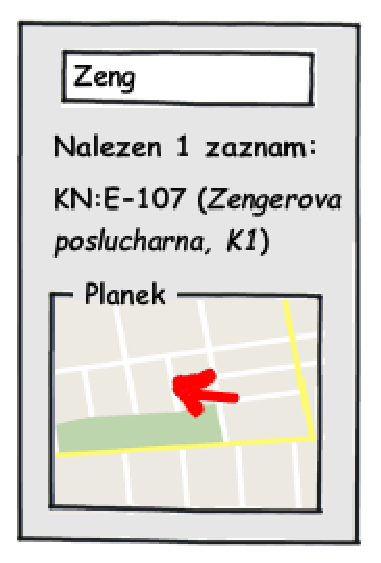
\includegraphics[width=30mm]{figures/LFjedinyVysledek}
\caption{Nalezení jediného výsledku}
\label{fig:LFjedinyVysledek}
\end{center}
\end{figure}

Aplikace by ještě měla poskytovat rozšířené vyhledávání s upřesněním hledaných míst a~zadáním výchozího bodu.

\noindent\textbf{Ostatní low fidelity prototypy jsou na přiloženém CD.}



\subsection{High fidelit prototyp}
High fidelity prototypy jsou už sofistikovanějšími prototypy, jejich vytvoření tudíž trvá déle, ale přesto se je vyplatí udělat před finální aplikací -- nemají totiž plnou funkčnost konečné aplikace, nemusí ošetřovat vstupy a řešit nestandardní situace, takže se pořád vytvoří relativně rychle, přičemž už zadavateli dokáží realisticky demonstrovat finální práci s aplikací.

High fidelity prototyp jsem vytvořil pomocí XHTML, ECMAScriptu a CSS. Jedná se o~velmi vhodné technologie pro tvorbu prototypů -- rychle se vytvoří a snadno se pak upravují. Testování takto vytvořených prototypů je také příjemné -- v případě v prototypu nevyřešené situace lze snadno připravit výslednou situaci a testerovi ji na dálku bez nějakých komplikací podstrčit.

Na obrázku \ref{fig:HFviceVysledku} je vidět high fidelity prototyp ve stavu zobrazení více výsledků vyhledání.

\begin{figure}[ht]
\begin{center}
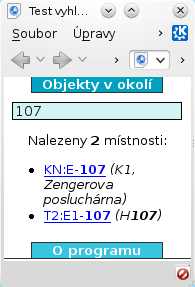
\includegraphics[width=30mm]{figures/HFviceVysledku}
\caption{Nalezení několika výsledku}
\label{fig:HFviceVysledku}
\end{center}
\end{figure}

Testování high fidelity prototypů je hlouběji popisované v kapitole o testování (viz \ref{sec:testhfp}).

\noindent\textbf{High fidelity prototyp je na přiloženém CD.}



\section{Případy užití}
Případy užití (use cases) jsou scénáře popisující chování systému z pohledu vnějšího aktéra. Případy užití vymezují, kdo a co bude jak dělat a z tohoto základu se později sestaví funkční požadavky. Už ze zadání aplikace vyplývá potřeba jediného aktéra -- studenta. Základní případy užití jsou následující:
\subsection{UC1: Hledání místnosti podle označení}
\label{ssec:UChledaniMistnosti}
\begin{description}
\item[Aktéři:] Student.
\item[Systém:] Navigační aplikace.
\item[Vstupní podmínky:] ~\\*[-1.5em]
 \begin{itemize}
 \item Student je ve výchozí obrazovce aplikace.
 \item Student se chce dostat do místnosti KN:E-9.
 \end{itemize}
\pagebreak
\item[Hlavní scénář:] ~\\*[-1.5em]
 \begin{enumerate}
 \item Student vstoupí do vyhledávacího formuláře.
 \item Student zadá písmeno \emph{K}.
 \item Aplikace zobrazí seznam místností obsahujících písmeno \emph{K}.
 \item Student zadá písmeno \emph{N}.
 \item Aplikace zobrazí seznam místností obsahujících výraz \emph{KN}.
 \item Student postupně zadá znaky \emph{:E-} a aplikace zúží seznam.
 \item Student zadá číslici \emph{9}.
 \item Aplikace zobrazí plán cílového patra s vyznačeným cílem.
 \item Student dojde podle plánu k cíli.
 \end{enumerate}
\item[Poznámky:] ~\\*[-1.5em]
 \begin{itemize}
 \item Místnost by mělo jít stejným způsobem vyhledat i podle starého číslování a zažitých názvů.
 \item Při zadání dvou a méně znaků lze kvůli nízkému výkonu zařízení a zachování přehlednosti zobrazovat upozornění na nutnost zadání více znaků.
 \end{itemize}
\end{description}

\subsection{UC2: Hledání neexistující místnosti}
\begin{description}
\item[Aktéři:] Student.
\item[Systém:] Navigační aplikace.
\item[Vstupní podmínky:] ~\\*[-1.5em]
 \begin{itemize}
 \item Student je ve výchozí obrazovce aplikace.
 \item Student se chce dostat do místnosti KN:X-777.
 \end{itemize}
\item[Hlavní scénář:] ~\\*[-1.5em]
 \begin{enumerate}
 \item Student vstoupí do vyhledávacího formuláře.
 \item Student postupně zadá znaky \emph{KN:X}.
 \item Aplikace sdělí studentovi, že místnost neexistuje.
 \end{enumerate}
\item[Poznámky:] ~\\*[-1.5em]
 \begin{itemize}
 \item Podrobný popis postupu zadávání znaků a reakcí aplikace je v UC1 \ref{ssec:UChledaniMistnosti}.
 \end{itemize}
\end{description}

\pagebreak
\subsection{UC3: Hledání kanceláře podle jména sídlícího vyučujícího}
\begin{description}
\item[Aktéři:] Student.
\item[Systém:] Navigační aplikace.
\item[Vstupní podmínky:] ~\\*[-1.5em]
 \begin{itemize}
 \item Student je ve výchozí obrazovce aplikace.
 \item Student chce nalézt kancelář Zdeňka Míkovce.
 \end{itemize}
\item[Hlavní scénář:] ~\\*[-1.5em]
 \begin{enumerate}
 \item Student vstoupí do vyhledávacího formuláře.
 \item Student zadá písmeno \emph{M}.
 \item Aplikace zobrazí seznam místností obsahujících písmeno \emph{M}.
 \item Student zadá písmeno \emph{í}.
 \item Aplikace zobrazí seznam místností obsahujících výraz \emph{Mí}.
 \item Student zadá písmeno \emph{k}.
 \item Aplikace zobrazí plán cílového patra s vyznačeným cílem.
 \item Student dojde podle plánu k cíli.
 \end{enumerate}
\end{description}

\subsection{UC4: Hledání nejbližšího nápojového automatu}
\begin{description}
\item[Aktéři:] Student.
\item[Systém:] Navigační aplikace.
\item[Vstupní podmínky:] ~\\*[-1.5em]
 \begin{itemize}
 \item Student je ve výchozí obrazovce aplikace.
 \item Student se chce dostat k nejbližšímu nápojovému automatu.
 \item Student se nachází před místností KN:E-9.
 \end{itemize}
\item[Hlavní scénář:] ~\\*[-1.5em]
 \begin{enumerate}
 \item Student vstoupí do vyhledávacího formuláře.
 \item Student vyhledá místnost KN:E-9 podle UC1 \ref{ssec:UChledaniMistnosti}.
 \item Aplikace zobrazí plán cílového patra s vyznačeným výchozím místem.
 \item Student v plánu vyhledá požadovaný nápojový automat.
 \item Student dojde podle plánu k cíli.
 \end{enumerate}
\end{description}

\subsection{UC5: Hledání za pomoci regulárních výrazů}
\begin{description}
\item[Aktéři:] Student.
\item[Systém:] Navigační aplikace.
\item[Vstupní podmínky:] ~\\*[-1.5em]
 \begin{itemize}
 \item Student je ve výchozí obrazovce aplikace.
 \item Student se chce dostat do místnosti KN:E-9.
 \end{itemize}
\item[Hlavní scénář:] ~\\*[-1.5em]
 \begin{enumerate}
 \item Student vstoupí do vyhledávacího formuláře.
 \item Student zadá znak \emph{-}.
 \item Aplikace zobrazí seznam místností obsahujících znak \emph{-}.
 \item Student zadá číslici \emph{9}.
 \item Aplikace zobrazí seznam místností obsahujících výraz \emph{-9}.
 \item Student zadá znak \emph{\$}.
 \item Aplikace zobrazí seznam místností končících výrazem \emph{-9}.
 \item Student si vybere ze seznamu místnost KN:E-9.
 \item Aplikace zobrazí plán cílového patra s vyznačeným cílem.
 \item Student dojde podle plánu k cíli.
 \end{enumerate}
\end{description}



\section{Funkční požadavky na systém}
Ačkoliv někdy slouží funkční požadavky (functional requirements), tedy požadavky na konkrétní funkčnost systému nebo jeho komponenty, jako podklad pro vytvoření případů užití, v tomto případě se postupovalo opačně -- bylo potřeba nejprve zanalyzovat potencionální činnosti uživatelů a na jejich základě se vytvořily požadavky:
\subsection{FR1: Vyhledávání místností}
Aplikace bude umět vyhledat místnost podle označení (KN:E-107), starého označení (K1), jména (Zengerova posluchárna) a zažitého názvu (Solárium). Aplikace bude umět vyhledat místnost i podle jména sídlícího vyučujícího.
\subsection{FR2: Vyhledávání míst v okolí}
Aplikace umožní vyhledávat body zájmu v okolí zadaného umístění. Mezi body zájmu patří občerstvení, toalety, výtahy a podobně.
\subsection{FR3: Určení aktuální pozice}
Aplikace umožní uživateli určit aktuální pozici.
\subsection{FR4: Určení cílové pozice}
Aplikace umožní uživateli určit cílovou pozici.
\subsection{FR5: Navádění k cíli}
Aplikace vhodně navede uživatele k cíli: zobrazí mu cestu s vyznačenými orientačními body.
\subsection{FR6: Vyhledávání regulárními výrazy}
Aplikace umožní vyhledávat za pomoci vhodně implementovaných regulárních výrazů: nebudou neznalé uživatele omezovat a méně znalým musí být s výrazy nabídnuta pomoc.
\subsection{FR7: Vyhledávání bez rozlišování velikosti písmen}
Aplikace umožní vyhledávat bez rozlišování velikosti písmen.
\subsection{FR8: Vyhledávání bez diakritiky}
Aplikace umožní vyhledávat bez diakritiky.
\subsection{FR9: Vyhledávání s našeptáváním}
Aplikace bude při zadávání hledané fráze zobrazovat výsledky rovnou -- bez nutnosti se přesouvat na potvrzovací tlačítko.
\subsection{FR10: Nápověda}
Aplikace bude obsahovat nápovědu k užívání.
\subsection{FR11: O programu}
Aplikace bude obsahovat informace o programu: verzi, kontakt na podporu, odkaz na aktuální verzi a podobně.



\section{Nefunkční požadavky na systém}
Mezi nefunkční požadavky  (non-functional requirements) aplikace, tedy požadavky zaměřené na systém jako celek, místo na určitou funkčnost, především patří:
\subsection{NFR1: Použitelnost}
Aplikace bude zaměřena na uživatele a bude mu poskytovat co největší možnou použitelnost.
\subsection{NFR2: Efektivnost vyhledávání}
Aplikace bude efektivně vyhledávat i při velikém množství položek v databázi -- nebude uživatele při používání omezovat rychlostí a bude mít přiměřené nároky na paměť zařízení.
\subsection{NFR3: Účinnost vizualizace}
Aplikace bude účinně vizualizovat výstup, aby se uživatel dostal k hledané informaci co nejmenším počtem kroků, ale aby měl zároveň přehled o obsahu právě zobrazovaného výstupu.
\subsection{NFR4: Multiplatformnost}
Aplikace bude provozovatelná na co nejširším počtu zařízení, zvláště mobilních.
\subsection{NFR5: Offline provoz}
Aplikace bude provozovatelná i bez připojení k Internetu, aby mohla být využívána také studenty bez datového připojení.
\subsection{NFR6: Svobodná licence}
Aplikace bude vytvořena pod GNU kompatibilní licencí, aby byl všem potencionálním zájemcům usnadněn její další rozvoj.



\section{Návrh řešení}
Návrh (design) této aplikace neprobíhal příliš dlouho, aplikace nemá být nijak složitá a~rozsáhlá, ani není po stránce návrhu nějak výjimečná, takže se zde návrhu příliš věnovat nebudeme.

\subsection{Vyhledávání}
Stěžejní funkcí má být vyhledávání, to je zároveň i stěžejním bodem návrhu. Je nutné splnit všechny funkční i nefunkční požadavky, kde je vyhledávání silně zastoupeno.

Vyhledávací algoritmus by měl fungovat následovně, začnu popisovat od databáze, ze které se vyhledává. Databáze bude obsahovat mnoho (až tisíce) záznamů a je proto v mobilním prostředí nutné, aby bylo vyhledávání, včetně samotné databáze, optimalizované. Aby došlo v průběhu vyhledávání ke snížení toku dat algoritmem, provedeme dekompozici databáze a vyčleníme hledatelné položky (označení učeben, jména vyučujících...) stranou, můžeme je ještě abecedně seřadit. Tady optimalizace databáze prozatím končí a můžeme se přesunout k samotnému algoritmu.

Původně jsem zamýšlel vyhledávat binárním půlením nebo jiným algoritmem optimalizovaným pro seřazený seznam, přišel ale požadavek na vyhledávání pomocí regulárních výrazů a tím tato možnost odpadla -- je potřeba projít všechny místnosti a zkontrolovat každou položku.

Regulární výrazy se nám většinou postarají i o nerozlišování velikosti písmen, takže si jimi alespoň pomůžeme k dalšímu požadavku.

Při kontrole položky můžeme zároveň vyřešit i požadavek na hledání bez diakritiky, zase ale musíme optimalizovat. Nebylo by složité vytvořit algoritmus, který zkouší nahradit každé písmeno bez diakritiky jeho diakritickými variantami, tím by nám ale výrazně narostla náročnost algoritmu, slovo \emph{mistnost} by tak najednou odpovídalo sto dvaceti osmi výrazům (\emph{mistnost}, \emph{m\textbf{í}stnost}, \emph{mi\textbf{š}tnost}, \emph{m\textbf{íš}tnost}...), tolikrát ale nezvládneme se současným výkonem mobilních zařízení celou databázi prohledat.\footnote{V praxi není toto omezení tolik markantní, označení místností obsahuje spíše znaky bez diakritiky. Vyhledávané osoby ale diakritiku ve jménech mají, takže toto omezení zachováme.} Umožníme vyhledávat buď jen s diakritikou, nebo bez, čímž slovo \emph{mistnost} bude odpovídat pouze dvěma výrazům (\emph{mistnost} a \emph{m\textbf{í}stnost}). Vyřešíme to následovně, všechny diakritiku obsahující položky v již dříve zmíněném duplicitním seznamu uložíme do tohoto seznamu ještě jednou, tentokrát bez diakritiky.

Nalezeným položkám přiřadíme místnosti, které reprezentují (například položce \emph{Josef Vomáčka} místnost \emph{KN:E-108}), vyřadíme duplicitní místnosti a seřadíme je podle abecedy.

\subsection{Navigace}
Zpočátku jsme v analýze uvažovali o vyznačení cesty z výchozího bodu do cílového, to by ale, mimo náročného algoritmu, dost uživateli v některých věcech přitížilo. V první řadě by přišel o mnoho místa malého displeje formulářem pro zadání výchozího bodu, v druhé řadě by bylo vytvoření optimálního algoritmu hledajícího cestu pravděpodobně nemožné (viz \ref{subs:UNcestaAplikaci}) a špatná cesta by se uživateli nemusela líbit. Problém v tom naštěstí pravděpodobně nebude, budovy nejsou stavěné jako bludiště a navigace po nich s plánkem není problém.

Vyhledáním místnosti získá aplikace cíl, ke kterému je potřeba uživatele navést. Dobrým řešením je ukázat uživateli plán cílového patra s vyznačeným cílem, orientačními body, schodišti (a výtahy) a vstupy do budovy (s~rozdíly pater). Uživatel se tak dokáže v plánu zorientovat, i kdyby se mu to doposud nepodařilo, schodiště (většinou vedou budovou každým patrem) a vchody do budovy (většinou jsou maximálně dva) k tomu velmi pomohou. Plán pouze cílového patra proto, že cestu po schodech nemá cenu vizualizovat (dokonce je to spíše nevhodné) a v rámci výchozího patra je většinou zcela zřejmé, jak se ke schodům dostat. Uživatel se tedy zvládne dostat do uvedeného patra a tam už podle plánu k hledané místnosti sám bez větších komplikací.
